\chapter{Einleitung}
\section{Motivation}\label{subsec:motivation}
``Digitalisierung des Handwerks'' - Das ist der Titel einer im Jahr 2017 ausgeführten Studie vom Branchenverband \textit{Bitkom}. 
Diese Studie besagt, dass 69\% der 509 befragten Handwerksbetriebe die Digitalisierung als Chance für einen positiven Umschwung der Betriebe sehen. 
Dabei ergeben sich aus Sicht der Handwerker die Vorteile von ``optimaler Lagerung und Logistik'' (91\%), ``Zeitersparnis'' (81\%) und ``flexibler Arbeitsorganisation'' (78\%) \citep{Bitkom17}. \\

Im November 2017 wurde in Hannover vom Güterschutzverband Stahlgerüstbau e.V. zum Thema ``Digitalisierung des Handwerks'' ein zweitägiges Groß-Seminar unter dem Titel ``Gerüstbau 4.0: Was bedeutet der digitale Wandel für den eigenen Betrieb?'' veranstaltet. 
Mit Vorträgen zu Themen wie ``Geschäftsprozesse im Gerüstbau-Handwerk'', ``Virtuelle Projekträume und Cloudlösungen'' und ``Mobile Datenverwaltung'' wurden die Teilnehmenden über den digitalen Wandel informiert \citep{GSV17}. \\

Der Gerüstbau-Dienstleister \emph{VERO Scaffolding EOOD Niederlassung Deutschland} aus Paderborn (nachfolgend: \vr{}) kann nach der Einführung und Benutzung einer selbst entwickelten Android-Applikation im Mai 2014 die genannten Vorteile der \textit{Bitkom}-Studie teilweise verzeichnen.
Die entwickelte App wird einerseits von den Monteuren zur Arbeitszeiterfassung, Einsicht von Auftragsinformationen und der Baustellendokumentation mit Fotos und Text genutzt.
Andererseits nutzt die Geschäfts- und Bauleitung die administrativen Funktionen der App, wie die Verwaltung und Pflege von Kunden-, Projekt-, und Arbeitsauftragsinformationen (siehe~\autoref{fig:app14}). \\

Zu diesen administrativen Aufgaben gehört auch die Aufmaßerfassung.
Die Aufmaßerfassung ist im Handwerk ein wichtiger Bestandteil als Vorbereitung zur Rechnungslegung.
Insbesondere im Gerüstbau, werden die Maße (Länge, Breite und Höhe) der bereitgestellten Gerüste abgemessen.
Meistens werden die Maße jedoch abgeschätzt und später im Büro erfasst und schließlich mit einer Preisliste nach Gerüsttyp (Fassadengerüst, Raumgerüst, Hängegerüst, etc.) abgerechnet.

\begin{figure}[h]
  \centering
  \begin{subfigure}[t]{0.3\textwidth}
    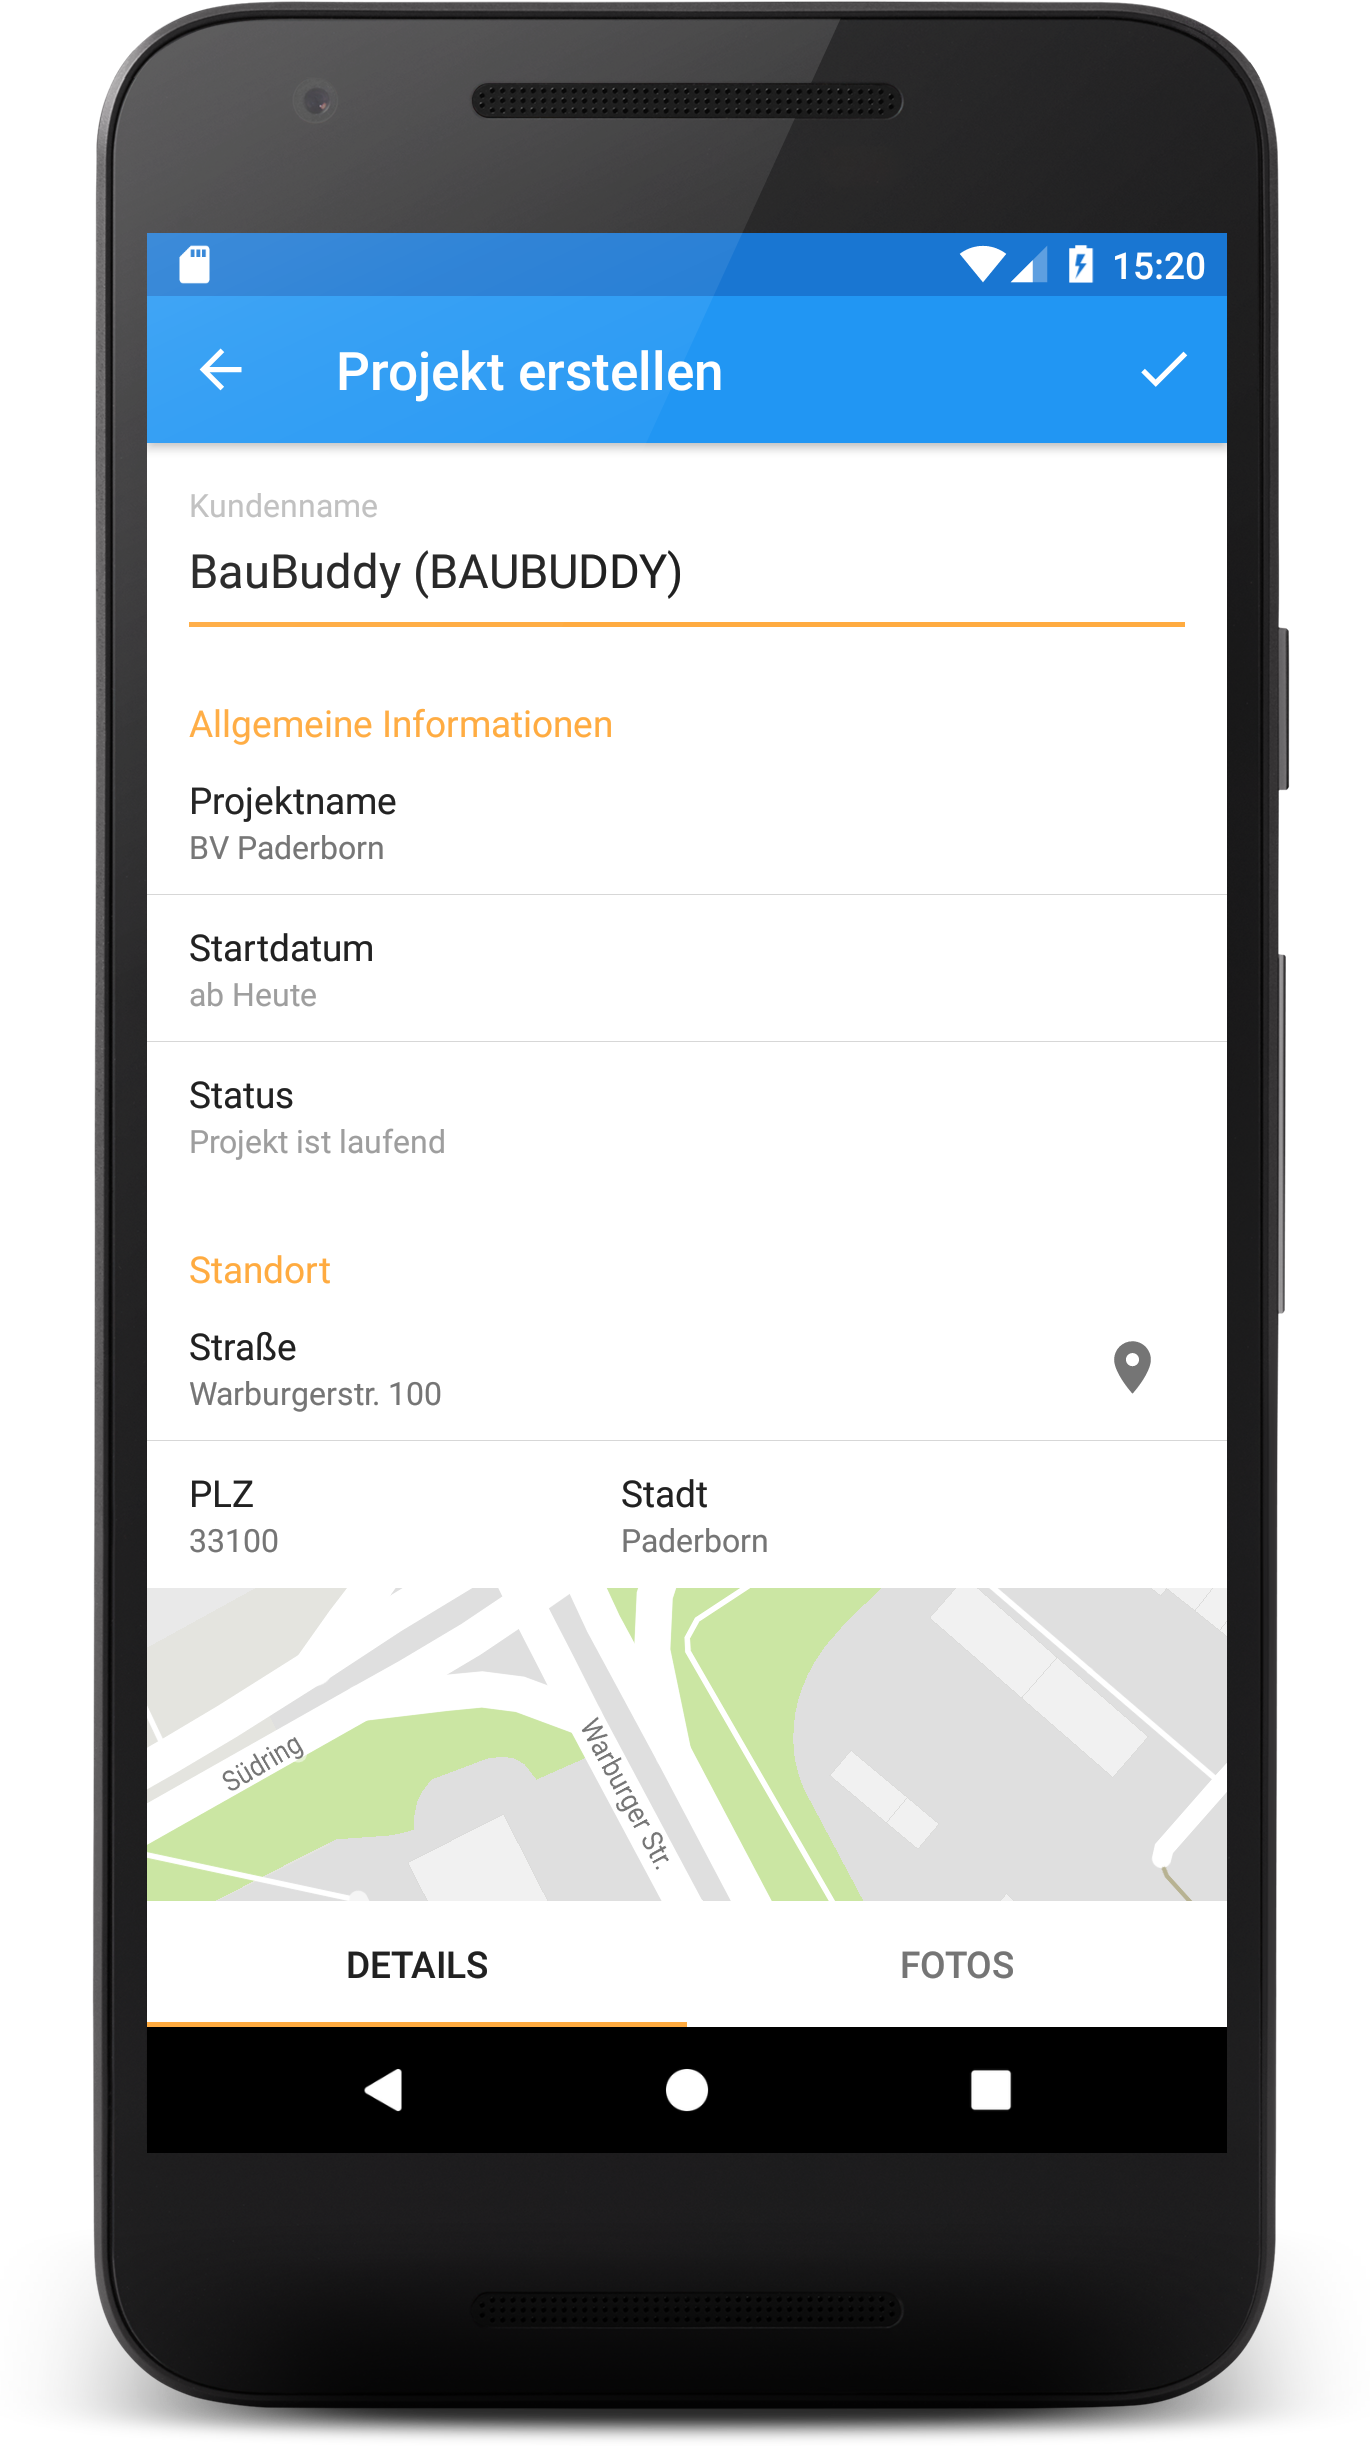
\includegraphics[keepaspectratio, width=\textwidth]{create_project}
    \caption{Erstellen eines neues Projekts}
  \end{subfigure}
  \begin{subfigure}[t]{0.3\textwidth}
    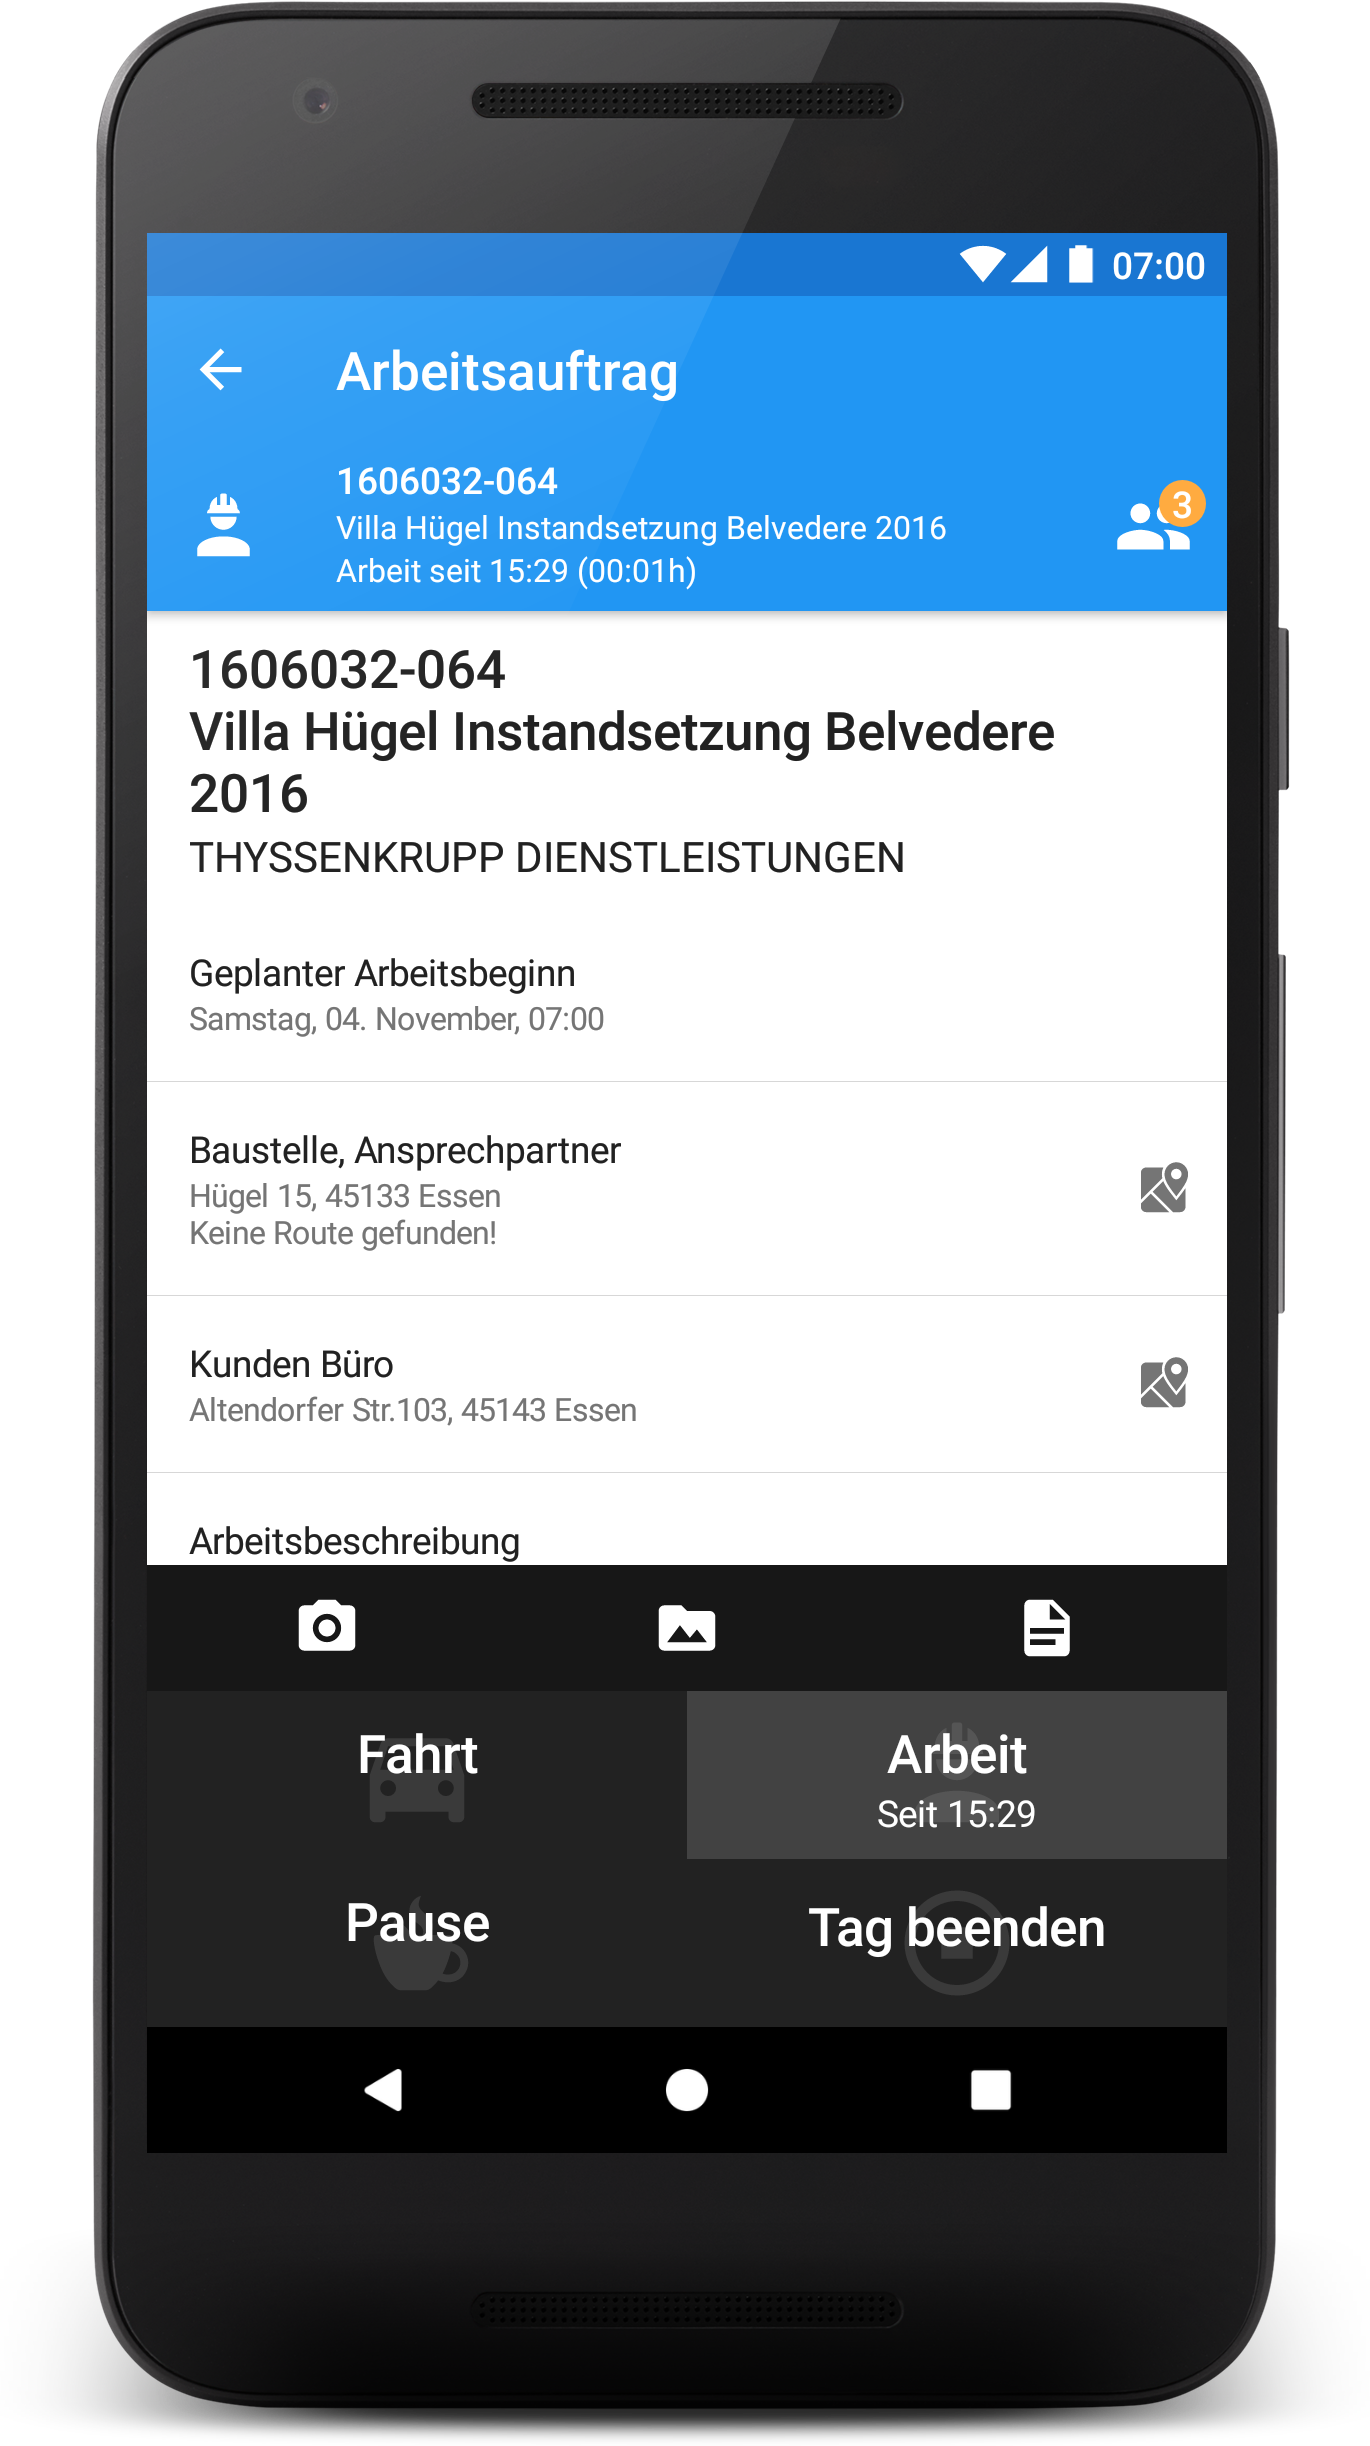
\includegraphics[keepaspectratio, width=\textwidth]{time_tracking}
    \caption{Arbeitszeiterfassung}
  \end{subfigure}
  \begin{subfigure}[t]{0.3\textwidth}
    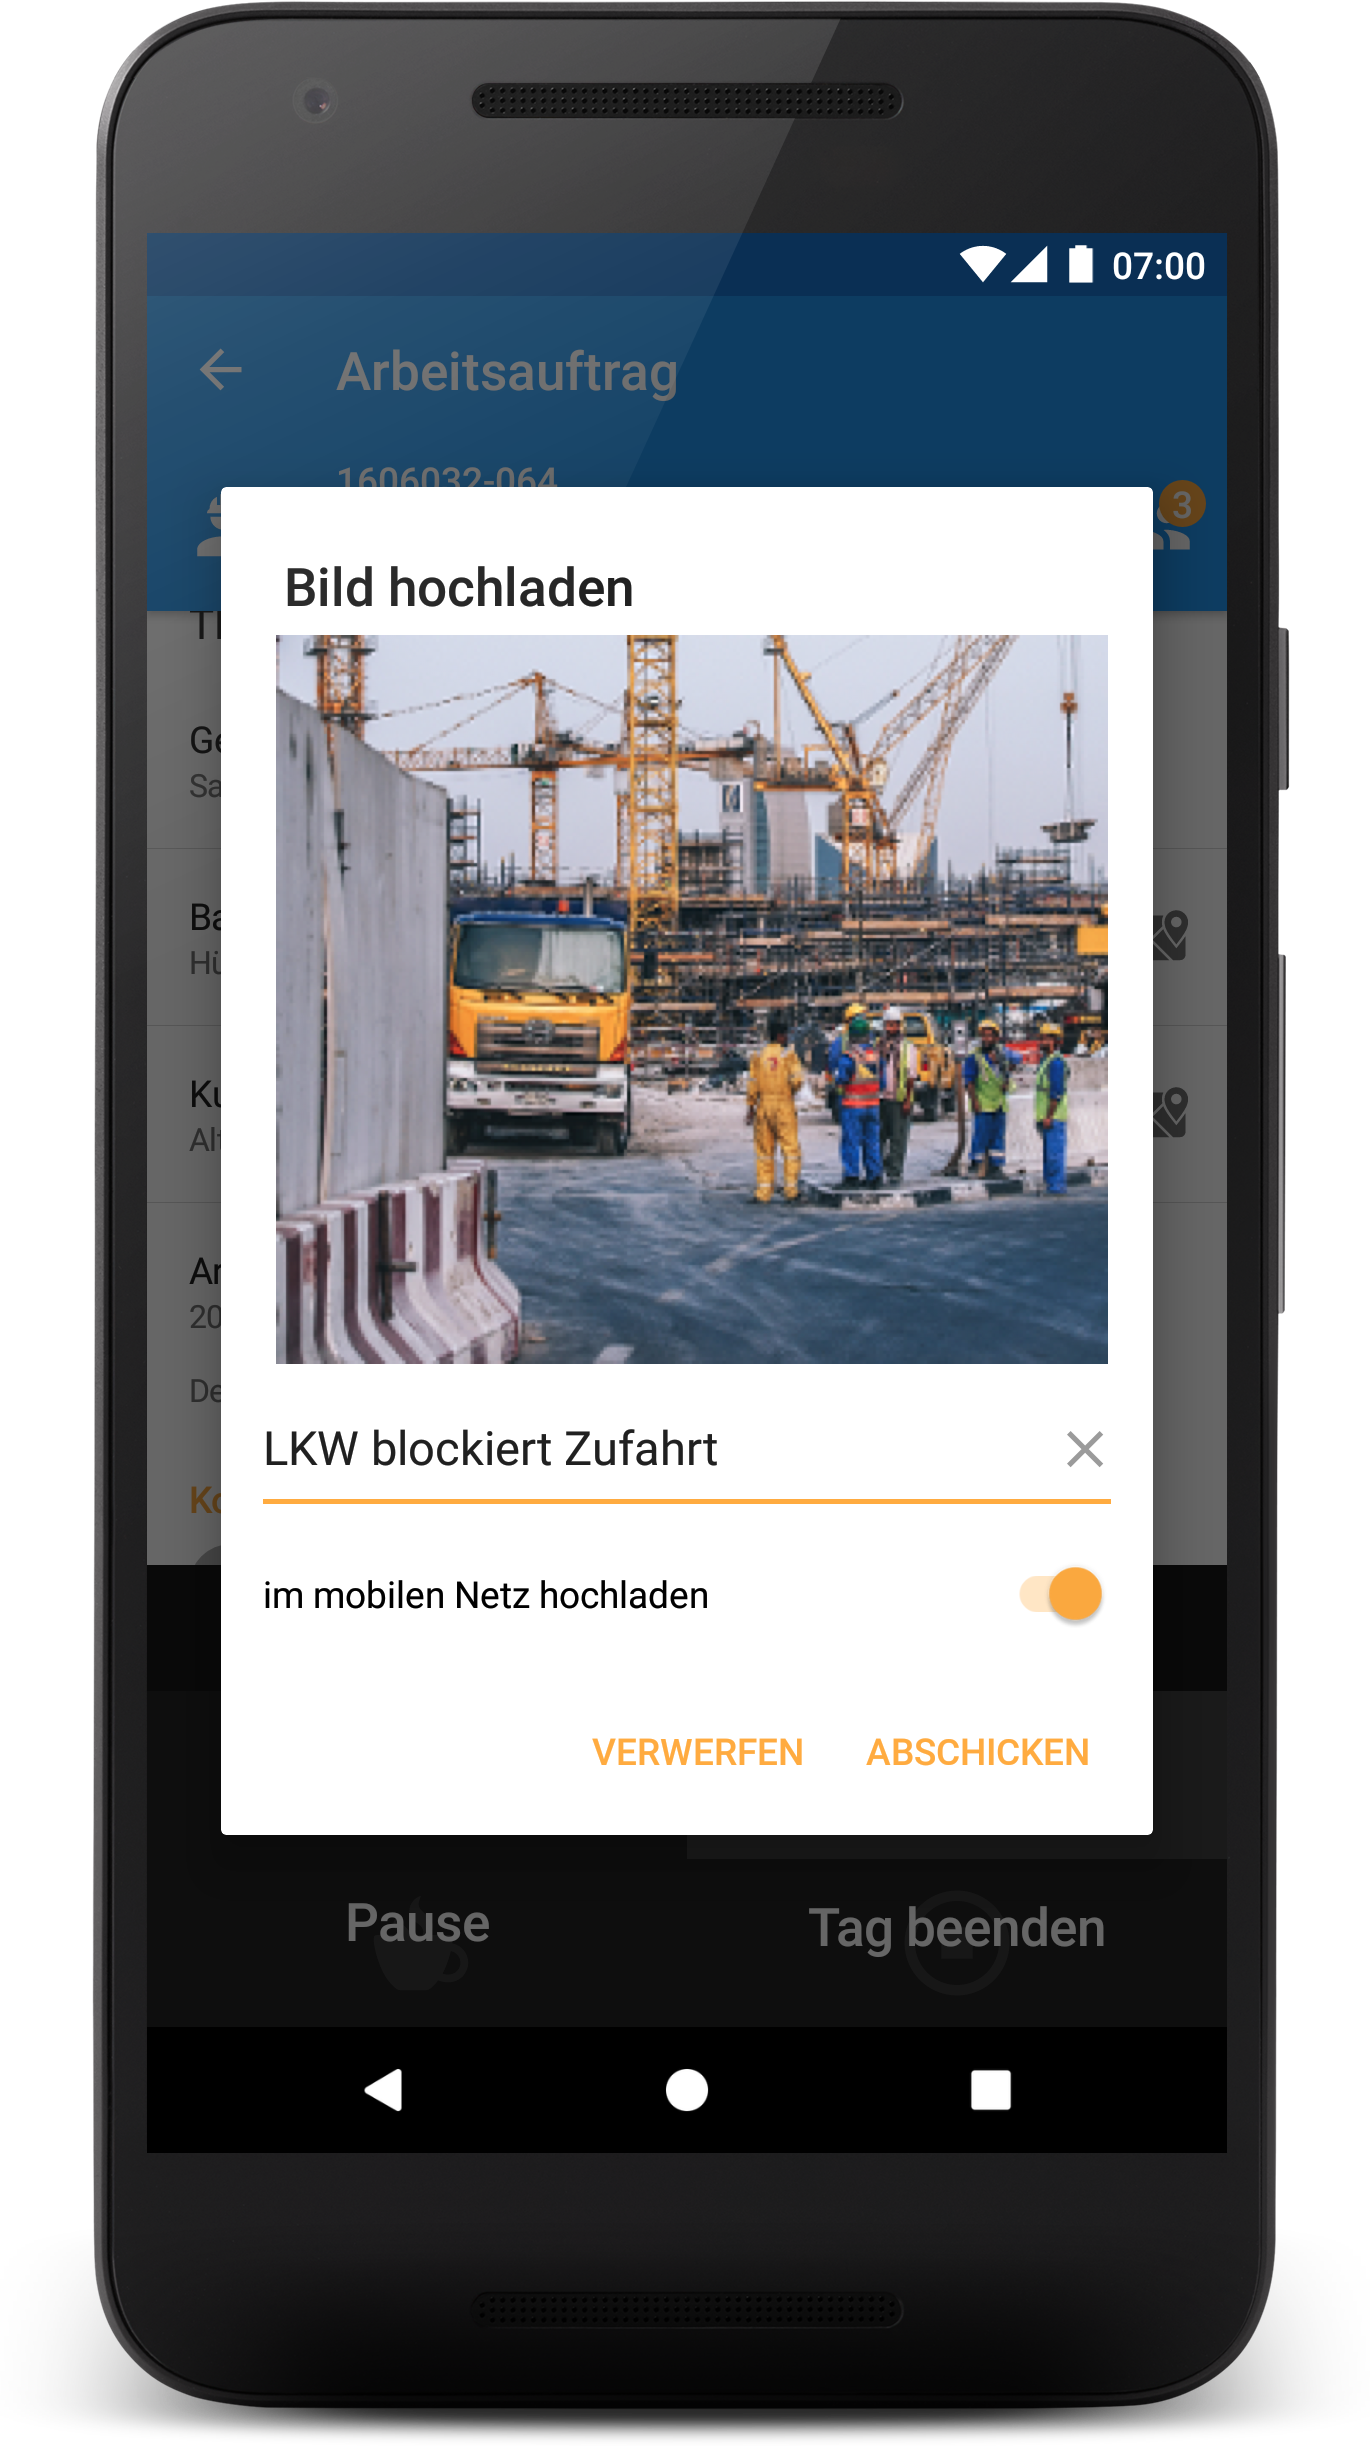
\includegraphics[keepaspectratio, width=\textwidth]{photo_docu}
    \caption{Fotodokumentation}
  \end{subfigure}
  \caption{Screenshots der ersten Funktionen der App (2014)}
  \label{fig:app14}
\end{figure}

\section{Umfeld}
Nach der Handwerkszählung vom statistischen Bundesamt im Jahr 2015 sind 13\% (75 264) aller Handwerksunternehmen dem Bauhauptgewerbe zuzuordnen.
Zu diesem Gewerbe zählt auch die Gerüstbaubranche, welche laut der Statistik überwiegend von kleinen Unternehmen dominiert wird (88,03\% der Unternehmen mit bis zu 20 Angestellten). 
9,28\% der Unternehmen verzeichnen zwischen 21 und 50 Beschäftigte und nur 2,69\% der Unternehmen verzeichnen über 50 Beschäftigte \cite{HZ17}.
Mit 14 Beschäftigten gehört die \emph{Fa.} \vr{} zu einem der kleineren Unternehmen in der Gerüstbaubranche.
Im Folgenden soll das Unternehmen und die selbst entwickelte Android-App vorgestellt werden.

\subsection{Unternehmen}
\vr{} geht aus der im Jahr $1999$ in Paderborn gegründeten \emph{VERO Gerüstbau GmbH} hervor. 
Seit 2013 ist die \emph{VERO Gerüstbau GmbH} die deutsche Niederlassung der bulgarischen \emph{VERO Scaffolding EOOD}, ansässig in Stara Zagora, Bulgarien.
Der Standort in Bulgarien fokussiert sich hauptsächlich auf mehrjährige Großprojekte in der Industrie (Kraftwerke, Raffinerien).
Der Fokus der deutschen Niederlassung in Paderborn liegt auf kleineren Projekten für Kommunen, Automobilzulieferer, aber auch private Haushalte.
Die Belegschaft am Standort Paderborn besteht aus zehn Monteuren, einem Auszubildenden, einer Bürofachkraft und zwei Geschäftsführern.
Die Monteure sind zwischen 19 und 55 Jahren alt und erledigen in zwei bis vier Kolonnen bis zu vier Arbeitsaufträge am Tag.

\subsection{Android-App und Systemarchitektur}
Im Oktober 2013 begann die Entwicklung einer Android-Applikation (nachfolgend: App) als mobile Software-Lösung für administrative Aufgaben der Monteure wie das Erfassen von Arbeitszeiten, Ansehen von Arbeitsaufträgen und das Verfassen von schriftlichen Baudokumentationen.
Die App kommuniziert zur Synchronisation der gesammelten Daten mit einer Server-Schnittstelle (\emph{API}\urlnote{https://www.gruenderszene.de/lexikon/begriffe/application-programming-interface-api}), welche auch von \vr{} entwickelt wurde.
Diese \emph{API} ist wiederum an eine SQL-Datenbank, ein Dateisystem und externe Dienste, wie einen E-Mail-Dienst, gekoppelt. \\

Im Vergleich zur anfänglichen Entwicklung aus dem Jahr 2013 verfügt die App zum jetzigen Stand (Januar 2018) über eine Vielzahl neuer Funktionen, die dem Nutzer den Arbeitsalltag erleichtern sollen (siehe \autoref{fig:app18}).
Hierzu zählt zum Beispiel eine monatliche Stundenübersicht für die Mitarbeiter, die mobile Verwaltung von Stammdaten (wie etwa von Mitarbeitern und Fahrzeugen), sowie eine Vorplanungstafel, um Termine und Arbeitsaufträge übersichtlich zu planen. 

\begin{figure}[h]
  \centering
  \begin{subfigure}[t]{0.4\textwidth}
    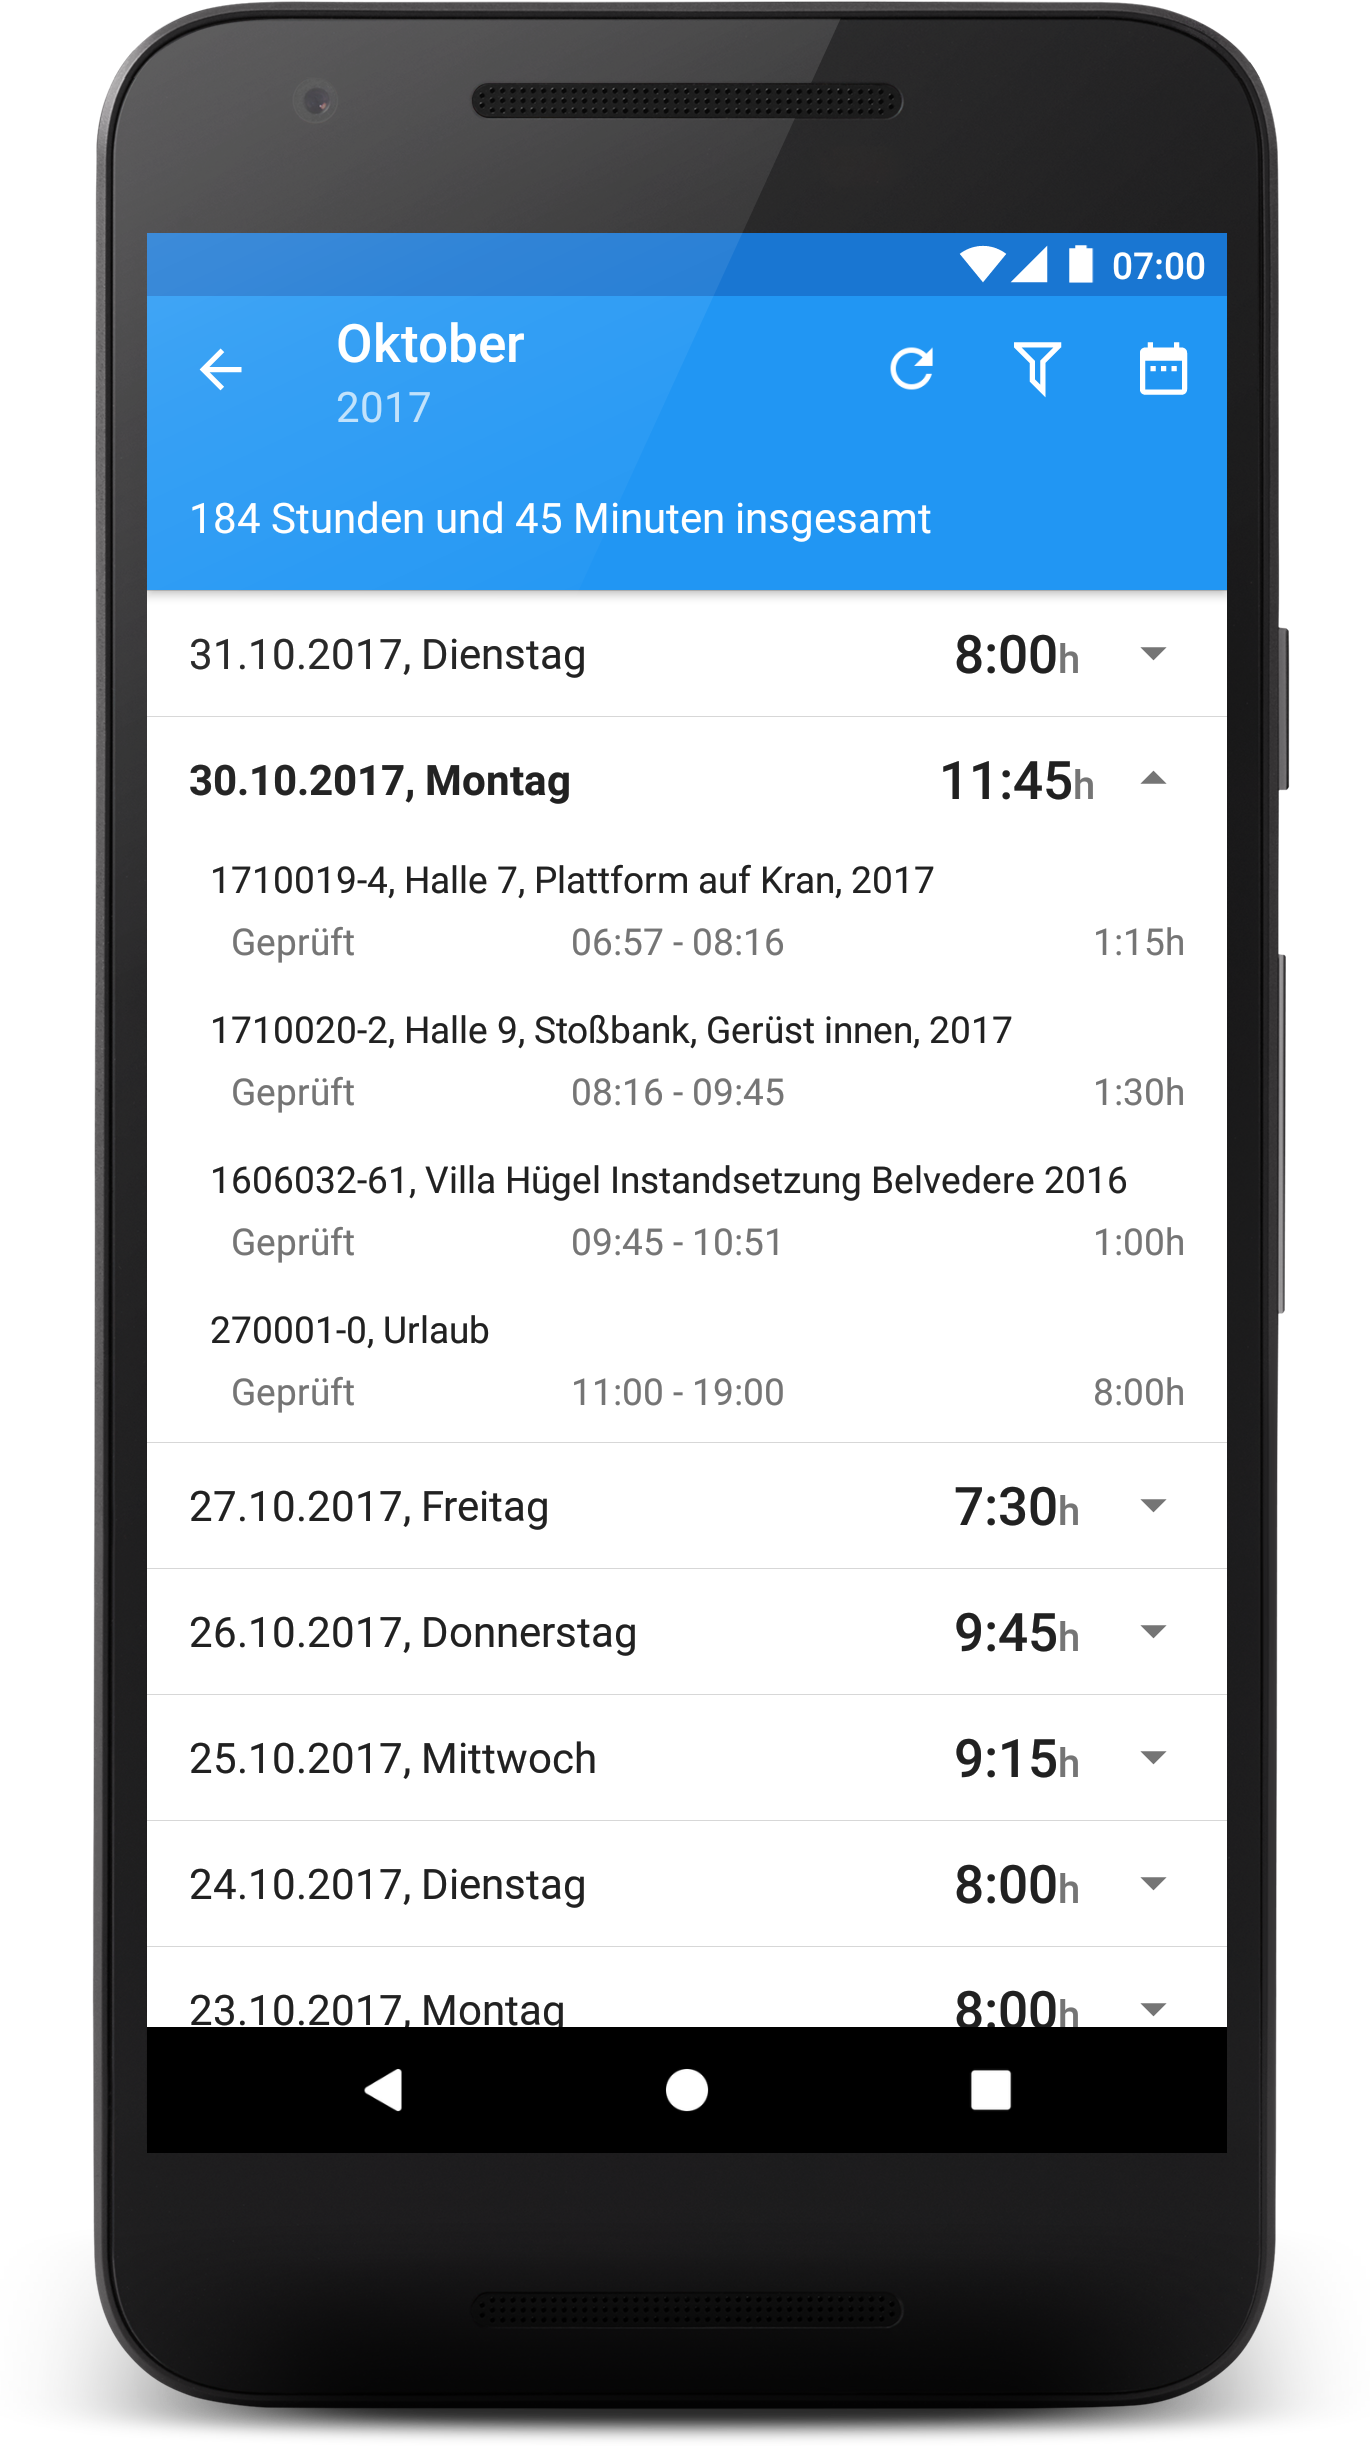
\includegraphics[keepaspectratio, width=\textwidth]{hours_overview}
    \caption{Monatliche Stundenübersicht}
  \end{subfigure}
  \begin{subfigure}[t]{0.4\textwidth}
    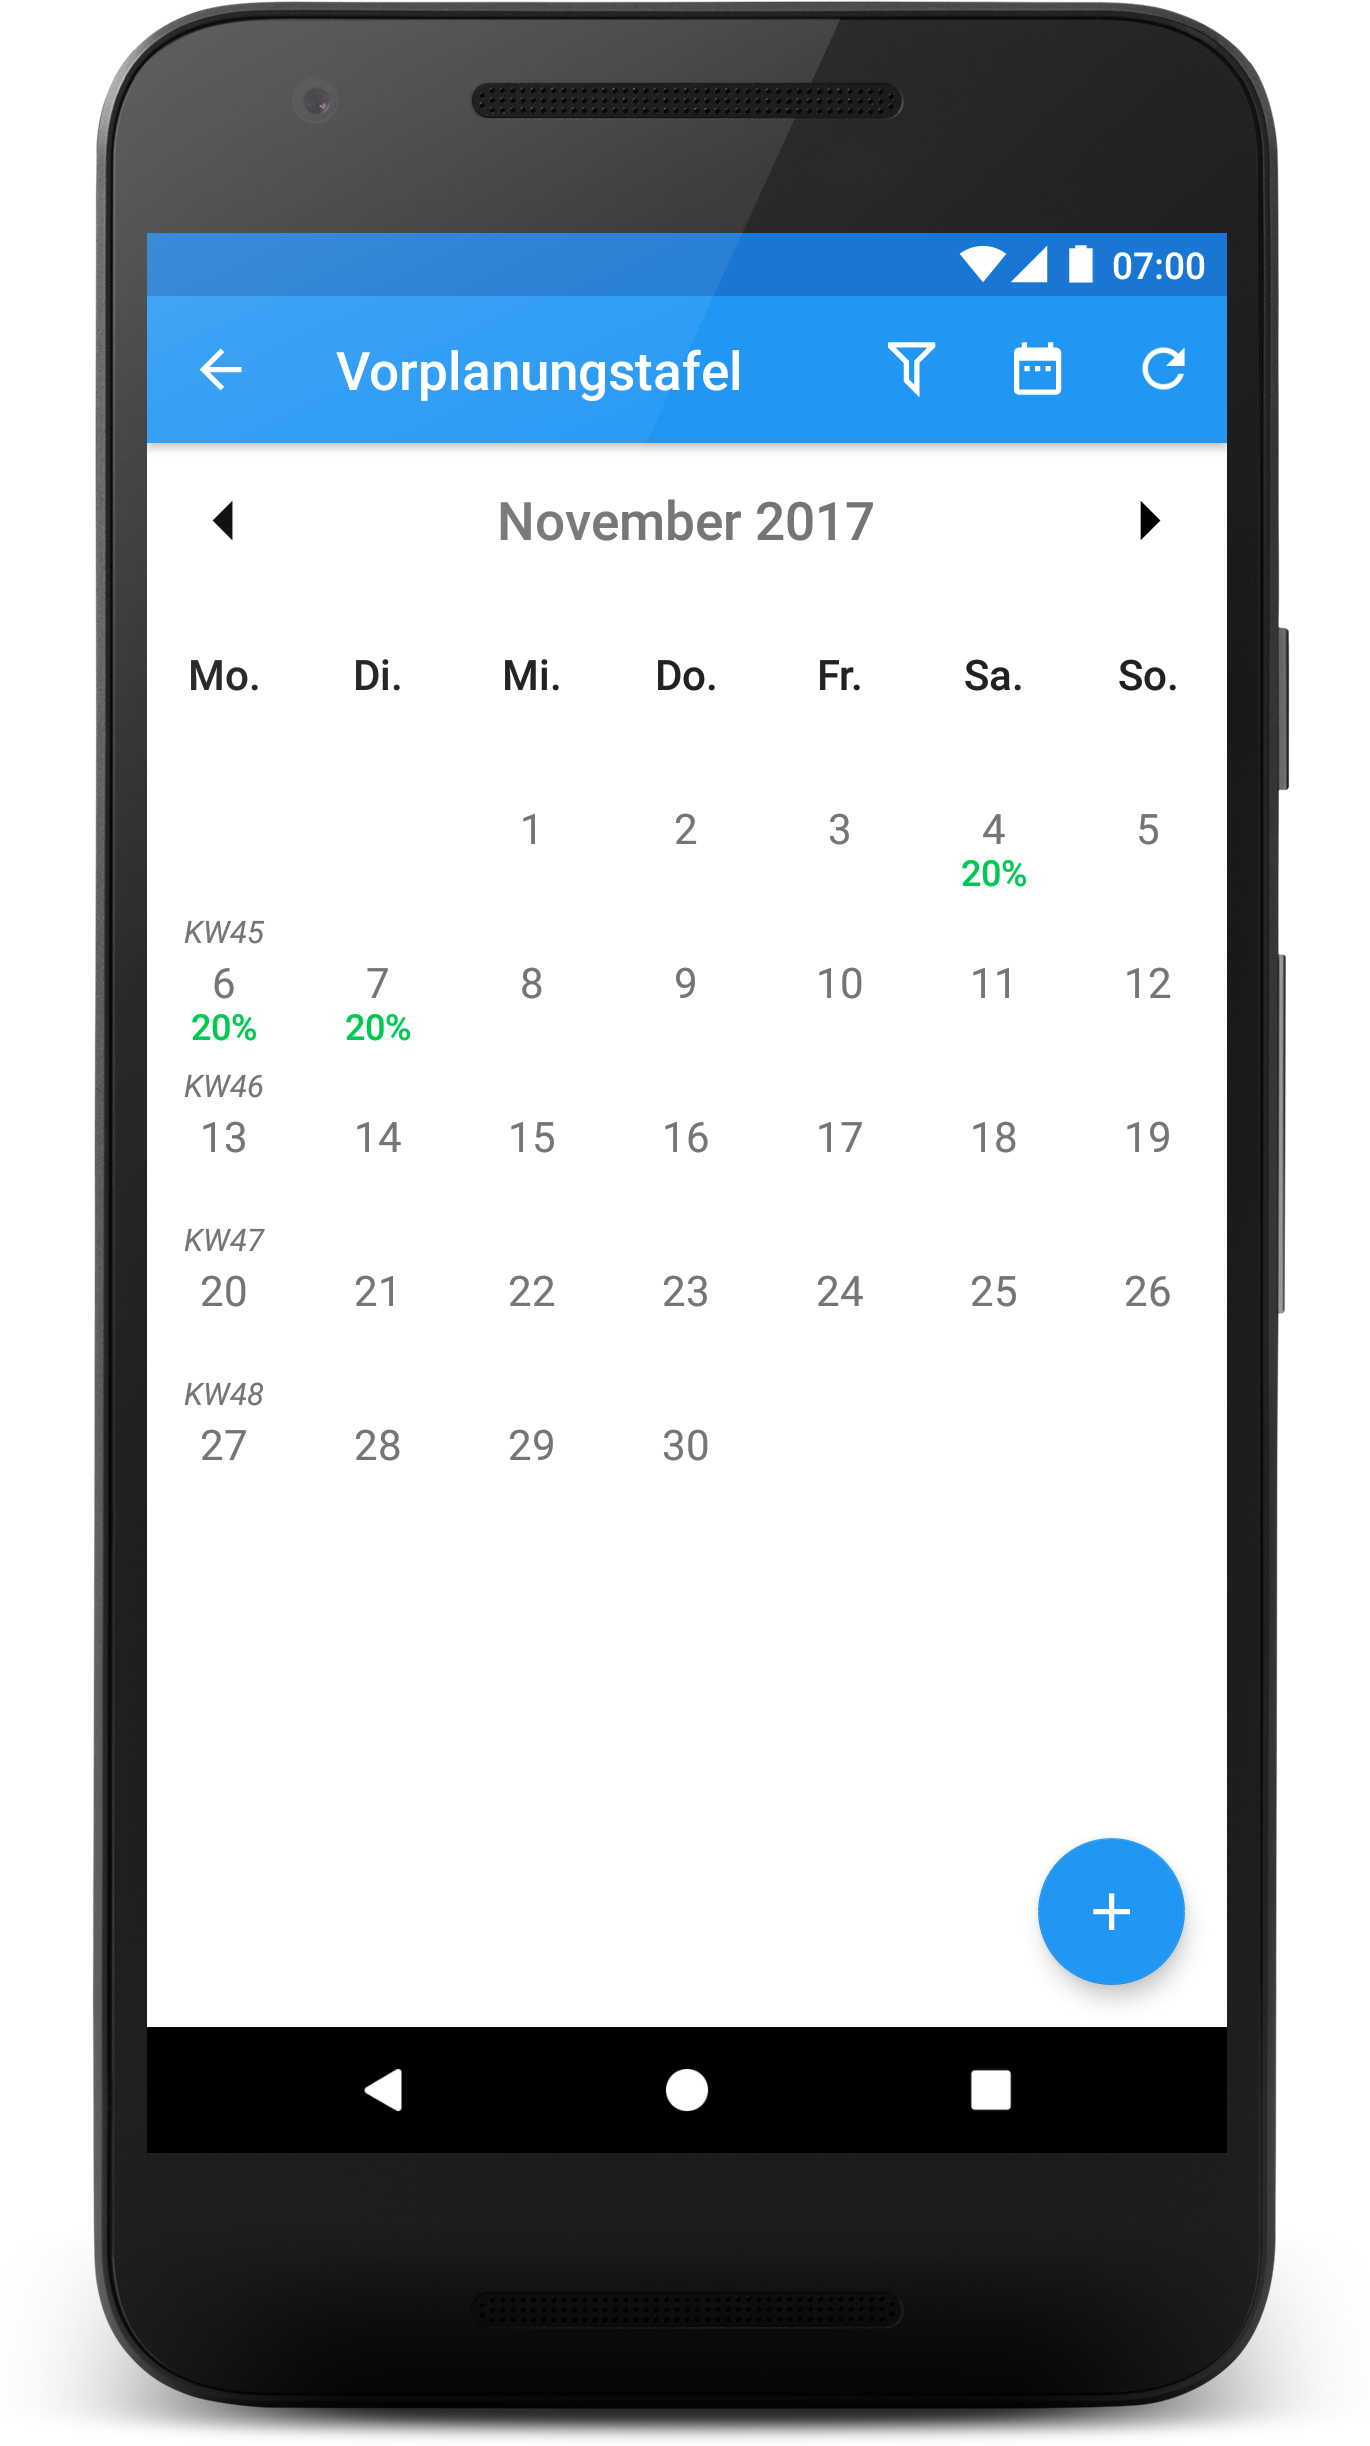
\includegraphics[keepaspectratio, width=\textwidth]{preplanning_board}
    \caption{Vorplanungstafel}
  \end{subfigure}
  \caption{Screenshots zweier neuen Funktionen der App (2018)}
  \label{fig:app18}
\end{figure}

\section{Ziel der Arbeit}
Im Rahmen dieser Arbeit soll die mobile Bildbearbeitung als effizienter Ansatz zur Aufmaßerfassung im Gerüstbau untersucht werden.
Ein Teilziel dieser Arbeit umfasst die Entwicklung einer App, welche in die bestehende Systemarchitektur der \emph{Fa.} \vr{} eingebunden werden soll.
Weiterhin soll die App den Monteuren ermöglichen, auf der Baustelle Aufmaße digital zu erfassen.
Hierbei soll insbesondere die intuitive Benutzung und positive Benutzererfahrung der App im Vordergrund stehen.
Wünschenswert wäre es zudem, am Ende dieser Arbeit eine gesteigerte Effizienz im Vergleich zum bisherigen analogen Prozess der Aufmaßerfassung verzeichnen zu können.

\section{Aufbau der Arbeit}
Eingangs wird die in dieser Arbeit angewandte Forschungsmethodik des \hcdp{} nach \citet{Norman13} in Kapitel 2 vorgestellt und die Anwendung in dieser Arbeit beschrieben. \\

Anschließend wird in Kapitel 3 der bisherige Prozess der Aufmaßerfassung im Gerüstbau am Beispiel der \emph{Fa.} \vr{} vorgestellt und die potentiellen Schwachstellen identifiziert. 
Infolgedessen wird ein möglicher, optimierter Prozess der Aufmaßerfassung beschrieben. \\

In Kapitel 4 werden zunächst Bewertungskriterien nach \citet{Nielsen94} zur Evaluation vorgestellt und gewichtet.
Nachfolgend werden drei Apps als mögliche Lösungsalternativen aus dem Google Play-Store vorgestellt und mittels der zuvor definierten Bewertungskriterien evaluiert.
Abschließend werden die Ergebnisse der Evaluation in einer Tabelle zum Vergleich aufbereitet. \\

Die Konzeption der eigenen Software-Lösung wird in Kapitel 5 weiter ausgeführt.
Zu den aus Kapitel 4 bekannten Kriterien werden praktischen Umsetzungsmöglichkeiten vorgestellt und diskutiert. \\

In Kapitel 6 wird die Implementierung eines ersten Prototyps beschrieben.
Dieser Prototyp wird anschließend in die bestehende Android-App eingebunden und für einen festgelegten Zeitraum von den Anwendern im Arbeitsalltag getestet.
Im Anschluss daran wird gemeinsam mit den Testpersonen der Prototyp evaluiert. \\

Basierend auf der Evaluation aus Kapitel 6 werden in den nachfolgenden Kapiteln 7, 8 und 9 drei weitere Iterationen des \hcdp{} durchgeführt.
Hier soll der Prototyp so weit verbessert werden, bis sich keine weiteren Usability-Probleme identifizieren lassen. \\

In Kapitel 10 werden eventuelle Probleme und Grenzen aufgezeigt und bewertet, die während den Iterationen des \hcdp{} aufgefallen sind. \\

Abschließend wird in Kapitel 11 ausgewertet, ob es eine Verbesserung im Hinblick auf die Effizienz bei der Benutzung der Android-App zur Aufmaßerfassung im Vergleich zum traditionellen, analogen Prozess gibt.
